\section{Matrix cookbook}

This doesn't matter as much for analytic calculations, but is useful for implementing autodiff on tensors from scratch.

\url{http://www.math.uwaterloo.ca/~hwolkowi//matrixcookbook.pdf}


\section{Large-scale distributed training}

{\it Goyal et al. 2017}
%\cite{goyal2017accurate}

\begin{itemize}
  \item Key contribution: no loss in accuracy when training with large minibatch sizes up to 8192 images.
  \item Linear scaling rule for adjusting learning rates as a function of mini-batch size.  Concretely, when minibatch size is multipled by $k$, multiply the learning rate by $k$.
  \item Warmup scheme that overcomes optimization challenges early in training.  Specifically, use a {\it low constant} learning rate for the first few epochs of training.  For a large minibatch of size $kn$, train with the low learning rate of $\eta$ for the first 5 epochs and then return to the target learning rate of $\hat{\eta} = k \eta$.
  \item Update rule:
    \[
      \hat{w}_{t+1} = w_t - \hat{\eta} \frac{1}{kn} \sum_{j < k} \sum_{x \in \mathcal{B}_j} \nabla l (x, w_t).
    \]
\end{itemize}

\section{Hyperparameter optimization}

\subsection{Population-based training}

{\it Jaderberg et al. 2017}
%\cite{jaderberg2017population}

\begin{itemize}
  \item Key contribution: asynchronous optimization algorithm which uses a fixed computational budget to jointly optimize a population of models and their hyperparameters
  \item Schedule of hyperparameters (instead of fixing a set for the whole course of training)
  \item Sequential optimization: run multiple training runs (potentially with early stopping)
  \item Parallel random/grid search: train multiple models in parallel with different weight initializations + hyperparameters, with the view that one of the models will be optimized the best.
  \item Population based training: starts like parallel search, randomly sampling hyperparameters and weight initializations.  Each training run asynchronously evaluates its performance periodically.  Explores new hyperparameters by modifying the better model's hyperparameters, before training is continued.

\begin{figure}[H]
   \centering
   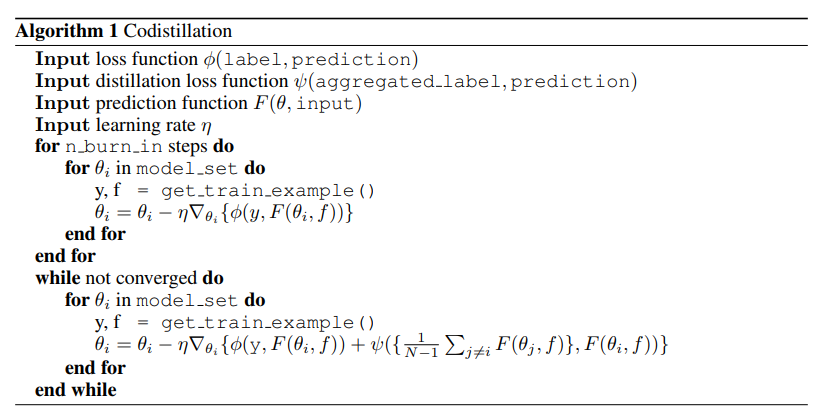
\includegraphics[width=\textwidth]{./img/pbt.png}
\end{figure}

\end{itemize}

\subsection{ENAS}

{\it Pham et al. 2018}
%~\cite{pham2018efficient}

\begin{itemize}
  \item Key contribution: fast + inexpensive approach for automatic model design.
  \item Controller (trained with policy gradient) discovers neural network architectures by searching for an optimal subgraph within a large computational graph.
  \item To train the shared parameters $\omega$ of the child models: we fix controller policy $\pi(\mbf{m}; \theta)$ and perform SGD on $\omega$ to minimize expected loss $\E_{\mbf{m} \sim \pi} [\mathcal{L} (\mbf{m}; \omega)]$.  Gradient is computed using Monte Carlo estimate
   \[ 
     \nabla_{\omega} \E_{\mbf{m} \sim \pi (\mbf{m}; \theta)} [\mathcal{L} (\mbf{m}; \omega)] \approx \frac{1}{M} \sum_{i=1}^{M} \nabla_{\omega} \mathcal{L}(\mbf{m}_i, \omega),
   \]
   where $\mbf{m}_i$ are sampled from $\pi(\mbf{m}; \theta)$.

 \item To train controller parameters $\theta$: fix $\omega$ and update $\theta$ to maximize the expected reward $\E_{\mbf{m} \sim \pi (\mbf{m}; \theta)} [\mathcal{R}(\mbf{m}, \omega)]$.  Use Adam optimizer, and compute the gradient with REINFORCE, with a moving average baseline to reduce variance.
\end{itemize}

\section{Distillation}

{\it Hinton et al. 2015}
%~\cite{hinton2015distilling}

\begin{itemize}
  \item Ensembling: train many different models on the same data and then average their prediction
  \item Distillation: compress the knowledge in an ensemble into a single model which is much easier to deploy.
\end{itemize}

{\it Anil et al. 2018}
%~\cite{anil2018large}

\begin{itemize}
  \item Online distillation enables extra parallelism.
  \item Codistillation algorithm:

\begin{figure}[H]
   \centering
   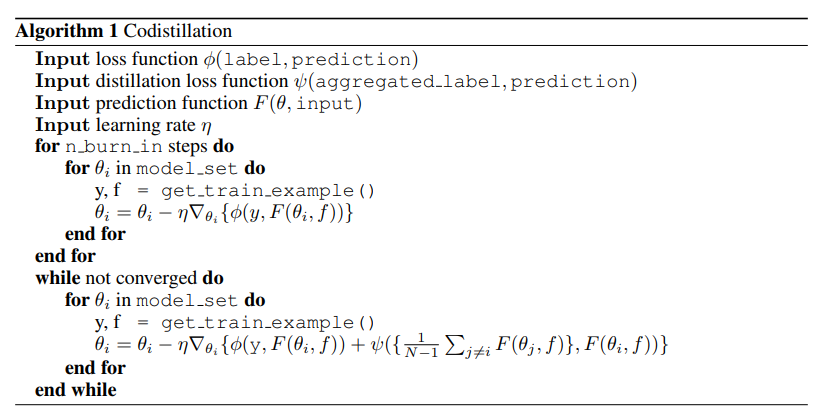
\includegraphics[width=\textwidth]{./img/codistillation.png}
\end{figure}

\end{itemize}


\section{ConvNet architectures}

\subsection{Recognition}
\begin{itemize}
  \item PNASNet-5-Large
    \begin{itemize}
      \item Similar to NAS, but performs search progressively (starting with models of low complexity).
    \end{itemize}
  \item NASNet-A-Large
    \begin{itemize}
      \item Uses a 50-step RNN as a controller to generate cell specifications.
    \end{itemize}
  \item SENet154
  \item PolyNet
\end{itemize}

\subsection{Detection}

\begin{itemize}
  \item Faster RCNN
  \item YOLO
  \item RetinaNet
\end{itemize}

\subsection{Segmentation}

\begin{itemize}
  \item FCNet
  \item DeepLabv4
  \item Dilated convolutions
\end{itemize}

\subsection{WaveNet}
Uses dilated convolutions:
  \begin{itemize}
      \item Let $F$ be a discrete function, and $k$ be a discrete filter.  The discrete convolution operator $*$ is defined as
        \[
          (F * k)(\mathbf{p}) = \sum_{\mathbf{s+t=p}} F(\mathbf{s}) k(\mathbf{t}).
        \]
        More generally, let $l$ be a dilation factor.  The $l$-dilated convolution can be defined as
        \[
          (F *_l k)(\mathbf{p}) = \sum_{\mathbf{s}+l\mathbf{t=p}} F(\mathbf{s}) k(\mathbf{t}).
        \]
      \item Implemented in TensorFlow as \texttt{tf.nn.atrous\_conv2d}
    \end{itemize}

\subsection{Self-attention networks}

\section{PyTorch}



\section{Backpropagation: CS231 intuitions}


\section{Backpropagation: a graph theory perspective}

Notes from Chris Olah's post: \url{http://colah.github.io/posts/2015-08-Backprop/}

Backpropagation is a very common algorithm, and is often referred to as ``reverse-mode differentation.''  At its core, it is a tool for calculating derivatives quickly.

Why are computational graphs a good abstraction?  To apply the multivariate chain rule:

\begin{enumerate}
  \item Sum over all possible paths from one node to the other.
  \item Multiply the derivatives on each edge of the path together.
\end{enumerate}

\subsection{Combinatorial explosion}

This is all just standard chain rule.  But how do you deal with cases like this?\footnote{Image source: Chris Olah.}

\begin{center}
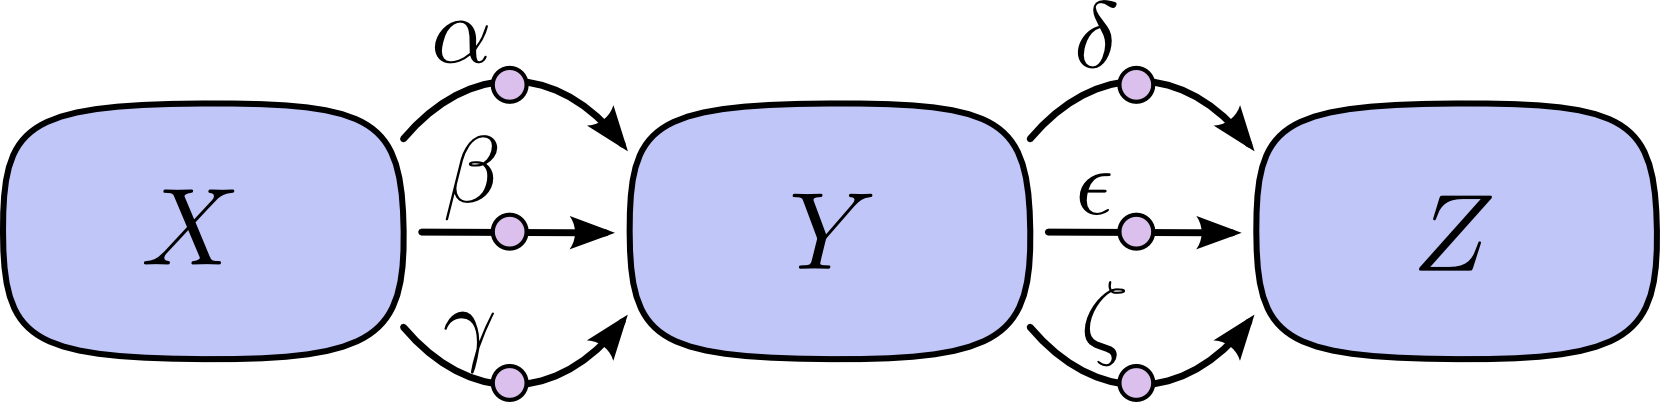
\includegraphics[width=0.5\textwidth]{img/chain-def-greek}
\end{center}

There are 9 paths in the above diagram.  Instead of naively summing over the paths, we can factor them:

\begin{align*}
  \frac{\partial Z}{\partial X} &= (\alpha + \beta + \gamma)(\delta + \varepsilon + \zeta).
\end{align*}

There are two algorithms we can leverage here.

\begin{enumerate}
  \item {\bf Forward-mode differentiation.} Start at an input to the graph, and move towards the end.  Sum all the paths feeding in.  The operator here is $\frac{\partial}{\partial X}$; similar to standard calculus.

    \begin{align*}
      \frac{\partial X}{\partial X} &= 1 \\
      \frac{\partial Y}{\partial X} &= \alpha + \beta + \gamma \\
      \frac{\partial Z}{\partial X} &= (\alpha + \beta + \gamma)(\delta + \varepsilon +\zeta).
    \end{align*}

  \item {\bf Reverse-mode differentiation.} Start at an output of the graph, and move towards the beginning.  At each node, merge all paths which started at that node.  The operator here is $\frac{\partial Z}{\partial }$.

    In particular:
    \begin{align*}
      \frac{\partial Z}{\partial Z} &= 1 \\
      \frac{\partial Z}{\partial Y} &= \delta + \varepsilon + \zeta  \\
      \frac{\partial Z}{\partial X} &= (\alpha + \beta + \gamma)(\delta + \varepsilon + \zeta) \\
    \end{align*}

\end{enumerate}

What is the difference between forward and reverse mode differentiation?  ``Forward-mode differentiation tracks how one input affects every node.''  ``Reverse-mode differentiation tracks how every node affects one output.''

\begin{align*}
  \T{forward mode: } &\frac{\partial}{\partial X} \\
  \T{reverse mode: } &\frac{\partial Z}{\partial}
\end{align*}

Reverse mode differtiation gives us the derivative of the output w.r.t. every node. This is exactly what we want.

On a large computational graph, this means reverse mode differentiation can get them all in one fell swoop.

In summary: derivatives are ridiculously computationally cheap.


\bibliographystyle{unsrt}
\bibliography{refs}
